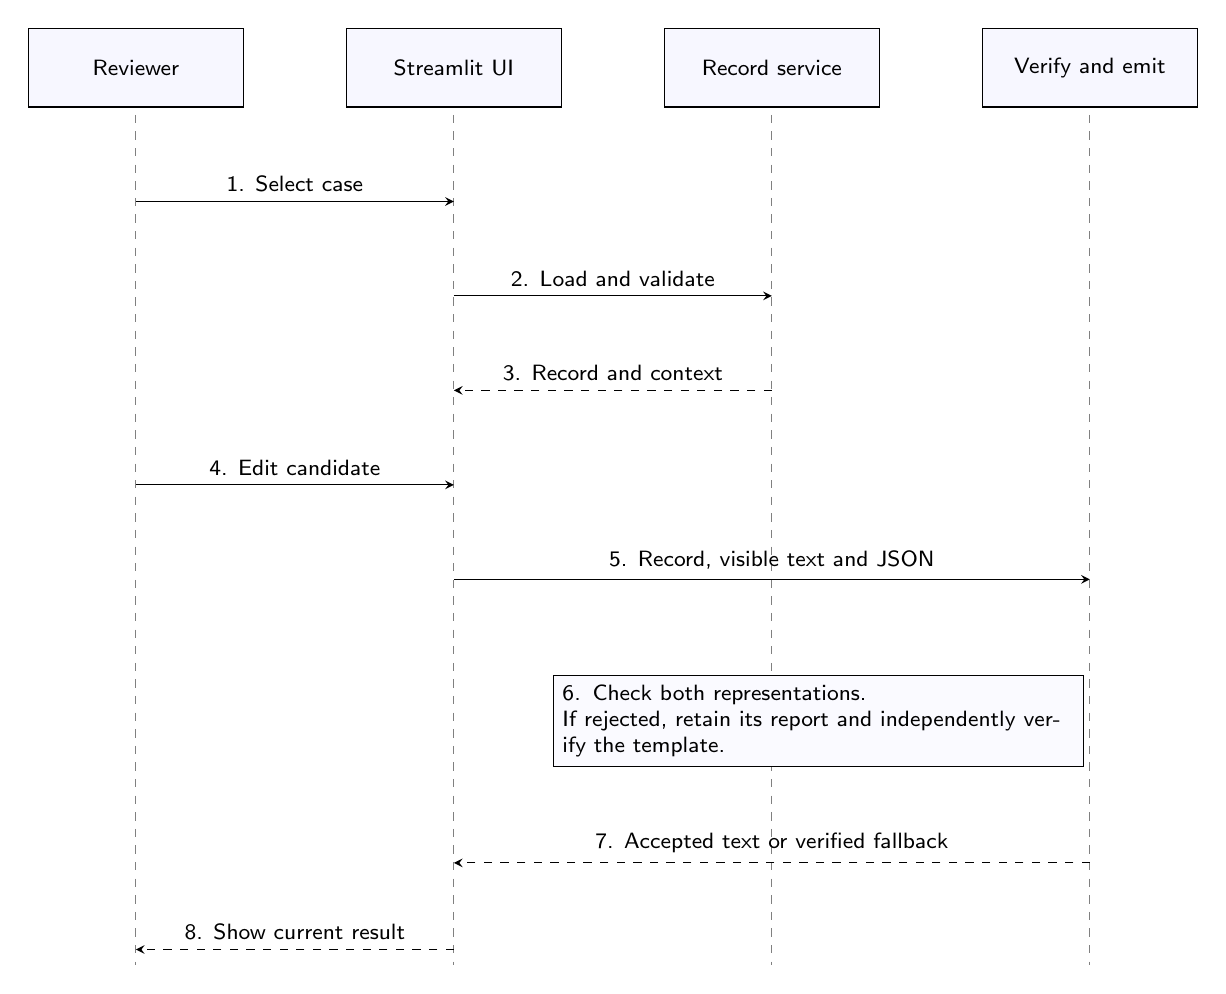
\begin{tikzpicture}[x=.985mm,y=1mm,font=\sffamily\footnotesize,>=stealth]
\foreach \x/\n in {12/Reviewer,53/Streamlit UI,94/Record service,135/Verify and emit}{
\node[draw,fill=blue!3,text width=25mm,align=center,minimum height=10mm] at (\x,122){\n};
\draw[dashed,gray] (\x,116)--(\x,8);}
\draw[->] (12,105)--node[above]{1. Select case}(53,105);
\draw[->] (53,93)--node[above]{2. Load and validate}(94,93);
\draw[->,dashed] (94,81)--node[above]{3. Record and context}(53,81);
\draw[->] (12,69)--node[above]{4. Edit candidate}(53,69);
\draw[->] (53,57)--node[above]{5. Record, visible text and JSON}(135,57);
\node[align=left,text width=65mm,fill=blue!2,draw] at (100,39){6. Check both representations.\\If rejected, retain its report and independently verify the template.};
\draw[->,dashed] (135,21)--node[above]{7. Accepted text or verified fallback}(53,21);
\draw[->,dashed] (53,10)--node[above]{8. Show current result}(12,10);
\end{tikzpicture}
